% Options for packages loaded elsewhere
\PassOptionsToPackage{unicode}{hyperref}
\PassOptionsToPackage{hyphens}{url}
%
\documentclass[
]{article}
\usepackage{amsmath,amssymb}
\usepackage{iftex}
\ifPDFTeX
  \usepackage[T1]{fontenc}
  \usepackage[utf8]{inputenc}
  \usepackage{textcomp} % provide euro and other symbols
\else % if luatex or xetex
  \usepackage{unicode-math} % this also loads fontspec
  \defaultfontfeatures{Scale=MatchLowercase}
  \defaultfontfeatures[\rmfamily]{Ligatures=TeX,Scale=1}
\fi
\usepackage{lmodern}
\ifPDFTeX\else
  % xetex/luatex font selection
\fi
% Use upquote if available, for straight quotes in verbatim environments
\IfFileExists{upquote.sty}{\usepackage{upquote}}{}
\IfFileExists{microtype.sty}{% use microtype if available
  \usepackage[]{microtype}
  \UseMicrotypeSet[protrusion]{basicmath} % disable protrusion for tt fonts
}{}
\makeatletter
\@ifundefined{KOMAClassName}{% if non-KOMA class
  \IfFileExists{parskip.sty}{%
    \usepackage{parskip}
  }{% else
    \setlength{\parindent}{0pt}
    \setlength{\parskip}{6pt plus 2pt minus 1pt}}
}{% if KOMA class
  \KOMAoptions{parskip=half}}
\makeatother
\usepackage{xcolor}
\usepackage[margin=1in]{geometry}
\usepackage{color}
\usepackage{fancyvrb}
\newcommand{\VerbBar}{|}
\newcommand{\VERB}{\Verb[commandchars=\\\{\}]}
\DefineVerbatimEnvironment{Highlighting}{Verbatim}{commandchars=\\\{\}}
% Add ',fontsize=\small' for more characters per line
\usepackage{framed}
\definecolor{shadecolor}{RGB}{248,248,248}
\newenvironment{Shaded}{\begin{snugshade}}{\end{snugshade}}
\newcommand{\AlertTok}[1]{\textcolor[rgb]{0.94,0.16,0.16}{#1}}
\newcommand{\AnnotationTok}[1]{\textcolor[rgb]{0.56,0.35,0.01}{\textbf{\textit{#1}}}}
\newcommand{\AttributeTok}[1]{\textcolor[rgb]{0.13,0.29,0.53}{#1}}
\newcommand{\BaseNTok}[1]{\textcolor[rgb]{0.00,0.00,0.81}{#1}}
\newcommand{\BuiltInTok}[1]{#1}
\newcommand{\CharTok}[1]{\textcolor[rgb]{0.31,0.60,0.02}{#1}}
\newcommand{\CommentTok}[1]{\textcolor[rgb]{0.56,0.35,0.01}{\textit{#1}}}
\newcommand{\CommentVarTok}[1]{\textcolor[rgb]{0.56,0.35,0.01}{\textbf{\textit{#1}}}}
\newcommand{\ConstantTok}[1]{\textcolor[rgb]{0.56,0.35,0.01}{#1}}
\newcommand{\ControlFlowTok}[1]{\textcolor[rgb]{0.13,0.29,0.53}{\textbf{#1}}}
\newcommand{\DataTypeTok}[1]{\textcolor[rgb]{0.13,0.29,0.53}{#1}}
\newcommand{\DecValTok}[1]{\textcolor[rgb]{0.00,0.00,0.81}{#1}}
\newcommand{\DocumentationTok}[1]{\textcolor[rgb]{0.56,0.35,0.01}{\textbf{\textit{#1}}}}
\newcommand{\ErrorTok}[1]{\textcolor[rgb]{0.64,0.00,0.00}{\textbf{#1}}}
\newcommand{\ExtensionTok}[1]{#1}
\newcommand{\FloatTok}[1]{\textcolor[rgb]{0.00,0.00,0.81}{#1}}
\newcommand{\FunctionTok}[1]{\textcolor[rgb]{0.13,0.29,0.53}{\textbf{#1}}}
\newcommand{\ImportTok}[1]{#1}
\newcommand{\InformationTok}[1]{\textcolor[rgb]{0.56,0.35,0.01}{\textbf{\textit{#1}}}}
\newcommand{\KeywordTok}[1]{\textcolor[rgb]{0.13,0.29,0.53}{\textbf{#1}}}
\newcommand{\NormalTok}[1]{#1}
\newcommand{\OperatorTok}[1]{\textcolor[rgb]{0.81,0.36,0.00}{\textbf{#1}}}
\newcommand{\OtherTok}[1]{\textcolor[rgb]{0.56,0.35,0.01}{#1}}
\newcommand{\PreprocessorTok}[1]{\textcolor[rgb]{0.56,0.35,0.01}{\textit{#1}}}
\newcommand{\RegionMarkerTok}[1]{#1}
\newcommand{\SpecialCharTok}[1]{\textcolor[rgb]{0.81,0.36,0.00}{\textbf{#1}}}
\newcommand{\SpecialStringTok}[1]{\textcolor[rgb]{0.31,0.60,0.02}{#1}}
\newcommand{\StringTok}[1]{\textcolor[rgb]{0.31,0.60,0.02}{#1}}
\newcommand{\VariableTok}[1]{\textcolor[rgb]{0.00,0.00,0.00}{#1}}
\newcommand{\VerbatimStringTok}[1]{\textcolor[rgb]{0.31,0.60,0.02}{#1}}
\newcommand{\WarningTok}[1]{\textcolor[rgb]{0.56,0.35,0.01}{\textbf{\textit{#1}}}}
\usepackage{longtable,booktabs,array}
\usepackage{calc} % for calculating minipage widths
% Correct order of tables after \paragraph or \subparagraph
\usepackage{etoolbox}
\makeatletter
\patchcmd\longtable{\par}{\if@noskipsec\mbox{}\fi\par}{}{}
\makeatother
% Allow footnotes in longtable head/foot
\IfFileExists{footnotehyper.sty}{\usepackage{footnotehyper}}{\usepackage{footnote}}
\makesavenoteenv{longtable}
\usepackage{graphicx}
\makeatletter
\def\maxwidth{\ifdim\Gin@nat@width>\linewidth\linewidth\else\Gin@nat@width\fi}
\def\maxheight{\ifdim\Gin@nat@height>\textheight\textheight\else\Gin@nat@height\fi}
\makeatother
% Scale images if necessary, so that they will not overflow the page
% margins by default, and it is still possible to overwrite the defaults
% using explicit options in \includegraphics[width, height, ...]{}
\setkeys{Gin}{width=\maxwidth,height=\maxheight,keepaspectratio}
% Set default figure placement to htbp
\makeatletter
\def\fps@figure{htbp}
\makeatother
\setlength{\emergencystretch}{3em} % prevent overfull lines
\providecommand{\tightlist}{%
  \setlength{\itemsep}{0pt}\setlength{\parskip}{0pt}}
\setcounter{secnumdepth}{-\maxdimen} % remove section numbering
\ifLuaTeX
  \usepackage{selnolig}  % disable illegal ligatures
\fi
\IfFileExists{bookmark.sty}{\usepackage{bookmark}}{\usepackage{hyperref}}
\IfFileExists{xurl.sty}{\usepackage{xurl}}{} % add URL line breaks if available
\urlstyle{same}
\hypersetup{
  pdftitle={Práctica dirigida 3},
  hidelinks,
  pdfcreator={LaTeX via pandoc}}

\title{Práctica dirigida 3}
\author{}
\date{\vspace{-2.5em}}

\begin{document}
\maketitle

{
\setcounter{tocdepth}{1}
\tableofcontents
}

\includegraphics[width=0.3\linewidth]{logoPUCP}

\textbf{FACULTAD DE CIENCIAS SOCIALES - PUCP}

\hypertarget{curso-pol-278---estaduxedstica-para-el-anuxe1lisis-poluxedtico-1-semestre-2024---1}{%
\subsection{\texorpdfstring{Curso: POL 278 - Estadística para el
análisis político 1 \textbar{} Semestre 2024 - 1
}{Curso: POL 278 - Estadística para el análisis político 1 \textbar{} Semestre 2024 - 1  }}\label{curso-pol-278---estaduxedstica-para-el-anuxe1lisis-poluxedtico-1-semestre-2024---1}}

\hypertarget{repaso}{%
\subsection{\texorpdfstring{\textbf{Repaso}}{Repaso}}\label{repaso}}

\hypertarget{e-government-survey-2022-the-future-of-digital-government}{%
\subsubsection{\texorpdfstring{\textbf{E-Government Survey 2022: The
Future of Digital
Government}}{E-Government Survey 2022: The Future of Digital Government}}\label{e-government-survey-2022-the-future-of-digital-government}}

La Encuesta de las Naciones Unidas sobre Gobierno Electrónico se ha
publicado cada dos años por el Departamento de Asuntos Económicos y
Sociales de las Naciones Unidas desde 2001. La Encuesta evalúa el estado
de desarrollo del gobierno electrónico de todos los Estados miembros de
las Naciones Unidas y, durante este tiempo, ha establecido un conjunto
de datos y análisis exhaustivos.

La evaluación mide el rendimiento del gobierno electrónico de los países
en relación con los demás, en lugar de ser una medición absoluta.
Reconoce que cada país debe decidir el nivel y la extensión de sus
iniciativas de gobierno electrónico de acuerdo con sus propias
prioridades nacionales de desarrollo y para lograr los Objetivos de
Desarrollo Sostenible. La Encuesta sirve como una herramienta de
referencia y desarrollo para que los países aprendan entre sí,
identifiquen áreas de fortaleza y desafíos en el gobierno electrónico y
moldeen sus políticas y estrategias. También tiene como objetivo
facilitar e informar las discusiones de los órganos
intergubernamentales, incluida la Asamblea General de las Naciones
Unidas, el Consejo Económico y Social y el Foro Político de Alto Nivel.

\begin{center}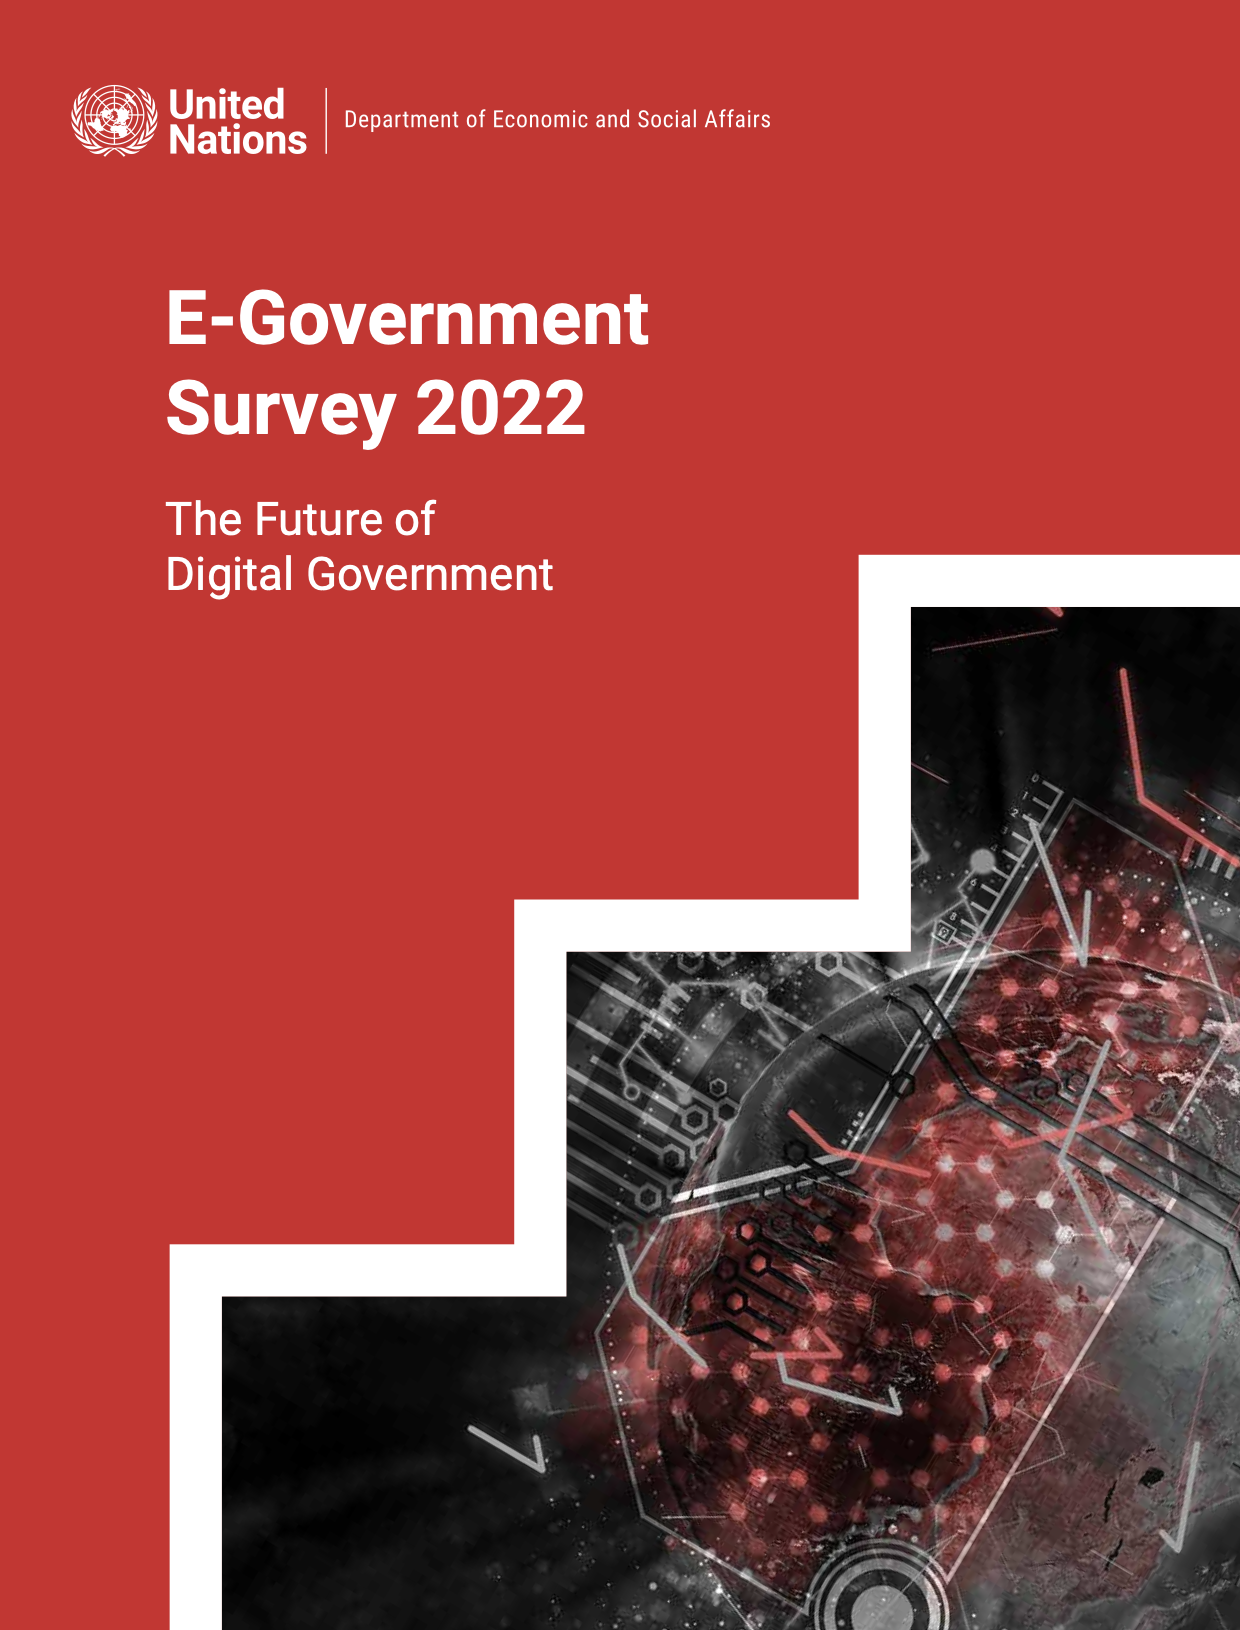
\includegraphics[width=0.5\linewidth]{PD3_egov22} \end{center}

Carguemos la data \emph{egov2022.xlsx}

\begin{Shaded}
\begin{Highlighting}[]
\FunctionTok{library}\NormalTok{(dplyr)}\CommentTok{\#Convocamos el paquete}
\FunctionTok{library}\NormalTok{(rio)    }
\NormalTok{data}\OtherTok{=}\FunctionTok{import}\NormalTok{(}\StringTok{"egov2022.xlsx"}\NormalTok{) }
\end{Highlighting}
\end{Shaded}

\begin{longtable}[]{@{}
  >{\raggedright\arraybackslash}p{(\columnwidth - 2\tabcolsep) * \real{0.3056}}
  >{\raggedright\arraybackslash}p{(\columnwidth - 2\tabcolsep) * \real{0.6944}}@{}}
\toprule\noalign{}
\begin{minipage}[b]{\linewidth}\raggedright
Nombre
\end{minipage} & \begin{minipage}[b]{\linewidth}\raggedright
Descripción
\end{minipage} \\
\midrule\noalign{}
\endhead
\bottomrule\noalign{}
\endlastfoot
Pais & Nombre del país \\
E\_gov & Indicador de gobernanza digital (0-100) \\
E\_part & Transparencia y acceso a la información, participación
ciudadana en línea (0 - 100) \\
Online\_service & Servicios en línea otorgado por el Estado (0-100) \\
Human\_cap & Miembros del Estado especializados en el tema (0-100) \\
Tele\_infra & Índice de capacidad de redes de telecomunicaciones como
acceso a internet 5G (0-100) \\
Alto\_teleinfra & ¿El país tiene un índice de infraestructura mayor a
80? Si/No \\
Region & Continente donde pertenece cada país \\
\end{longtable}

\hypertarget{recordando-el-anuxe1lisis-descriptivo}{%
\section{\texorpdfstring{\textbf{1.Recordando el análisis
descriptivo}}{1.Recordando el análisis descriptivo}}\label{recordando-el-anuxe1lisis-descriptivo}}

\begin{itemize}
\tightlist
\item
  \textbf{Moda}: Nominales, ordinales y numéricas
\item
  \textbf{Mediana}: Ordinales y numéricas
\item
  \textbf{Media}: Numéricas
\end{itemize}

Revisamos la estructura de la base de datos y sus variables

\begin{Shaded}
\begin{Highlighting}[]
\FunctionTok{str}\NormalTok{(data)}
\end{Highlighting}
\end{Shaded}

\begin{verbatim}
## 'data.frame':    181 obs. of  8 variables:
##  $ Pais          : chr  "Afghanistan" "Albania" "Algeria" "Andorra" ...
##  $ E_gov         : num  21 74 54 71 33 59 83 73 96 90 ...
##  $ E_part        : num  19 76 23 38 17 42 65 58 99 77 ...
##  $ Online_service: num  28 82 37 51 47 42 81 72 94 88 ...
##  $ Human_cap     : num  35 80 70 76 46 81 92 79 100 91 ...
##  $ Tele_infra    : num  19 60 61 88 20 60 73 69 88 85 ...
##  $ Alto_teleinfra: chr  "No" "No" "No" "Si" ...
##  $ Region        : chr  "Asia" "Europe" "Africa" "Europe" ...
\end{verbatim}

Podemos ver que casi todas las variables son numéricas, excepto la
variable \emph{Region} que se muestra como texto, pero es categórica.
Procedemos a revisar sus niveles y a recodificarla.

\begin{Shaded}
\begin{Highlighting}[]
\NormalTok{data }\SpecialCharTok{\%\textgreater{}\%} 
 \FunctionTok{group\_by}\NormalTok{(Region) }\SpecialCharTok{\%\textgreater{}\%} 
  \FunctionTok{summarize}\NormalTok{(}\AttributeTok{Freq=}\FunctionTok{n}\NormalTok{())}
\end{Highlighting}
\end{Shaded}

\begin{verbatim}
## # A tibble: 5 x 2
##   Region    Freq
##   <chr>    <int>
## 1 Africa      52
## 2 Americas    32
## 3 Asia        43
## 4 Europe      40
## 5 Oceania     14
\end{verbatim}

\begin{Shaded}
\begin{Highlighting}[]
\NormalTok{data}\SpecialCharTok{$}\NormalTok{Region}\OtherTok{=}\FunctionTok{as.factor}\NormalTok{(data}\SpecialCharTok{$}\NormalTok{Region)}
\FunctionTok{class}\NormalTok{(data}\SpecialCharTok{$}\NormalTok{Region) }\CommentTok{\#Comprobamos}
\end{Highlighting}
\end{Shaded}

\begin{verbatim}
## [1] "factor"
\end{verbatim}

\hypertarget{aplicaciuxf3n-en-r}{%
\section{\texorpdfstring{\textbf{2. Aplicación en
R}}{2. Aplicación en R}}\label{aplicaciuxf3n-en-r}}

\hypertarget{cuuxe1l-es-el-estado-de-la-gobernanza-digital-de-los-pauxedses}{%
\subsubsection{\texorpdfstring{\textbf{¿Cuál es el estado de la
gobernanza digital de los
países?}}{¿Cuál es el estado de la gobernanza digital de los países?}}\label{cuuxe1l-es-el-estado-de-la-gobernanza-digital-de-los-pauxedses}}

\begin{itemize}
\tightlist
\item
  \textbf{¿El país tiene un nivel alto de infraestructura en
  telecomunicaciones? (}Alto\_teleinfra) : Variable categórica
\end{itemize}

Realicemos una tabla de frecuencias de la variable:

\begin{Shaded}
\begin{Highlighting}[]
\NormalTok{para\_grafico}\OtherTok{=}\NormalTok{ data }\SpecialCharTok{\%\textgreater{}\%}
  \FunctionTok{group\_by}\NormalTok{(Alto\_teleinfra) }\SpecialCharTok{\%\textgreater{}\%} 
  \FunctionTok{summarise}\NormalTok{(}\AttributeTok{Freq=}\FunctionTok{n}\NormalTok{())}
\end{Highlighting}
\end{Shaded}

¿Qué nos indica la tabla? En este caso, ¿cuál sería la moda?

Revisemos en un gráfico:

\begin{Shaded}
\begin{Highlighting}[]
\FunctionTok{library}\NormalTok{(ggplot2)}
\FunctionTok{ggplot}\NormalTok{(para\_grafico, }\FunctionTok{aes}\NormalTok{(}\AttributeTok{x=}\NormalTok{Alto\_teleinfra, }\AttributeTok{y =}\NormalTok{ Freq, }\AttributeTok{fill=}\NormalTok{Alto\_teleinfra))}\SpecialCharTok{+}
  \FunctionTok{geom\_bar}\NormalTok{(}\AttributeTok{stat =} \StringTok{"identity"}\NormalTok{)}\SpecialCharTok{+} \FunctionTok{xlab}\NormalTok{(}\StringTok{"Alto nivel de infraestructura en telecomunicaciones"}\NormalTok{)}\SpecialCharTok{+}\FunctionTok{ylab}\NormalTok{(}\StringTok{"Frecuencia"}\NormalTok{)}
\end{Highlighting}
\end{Shaded}

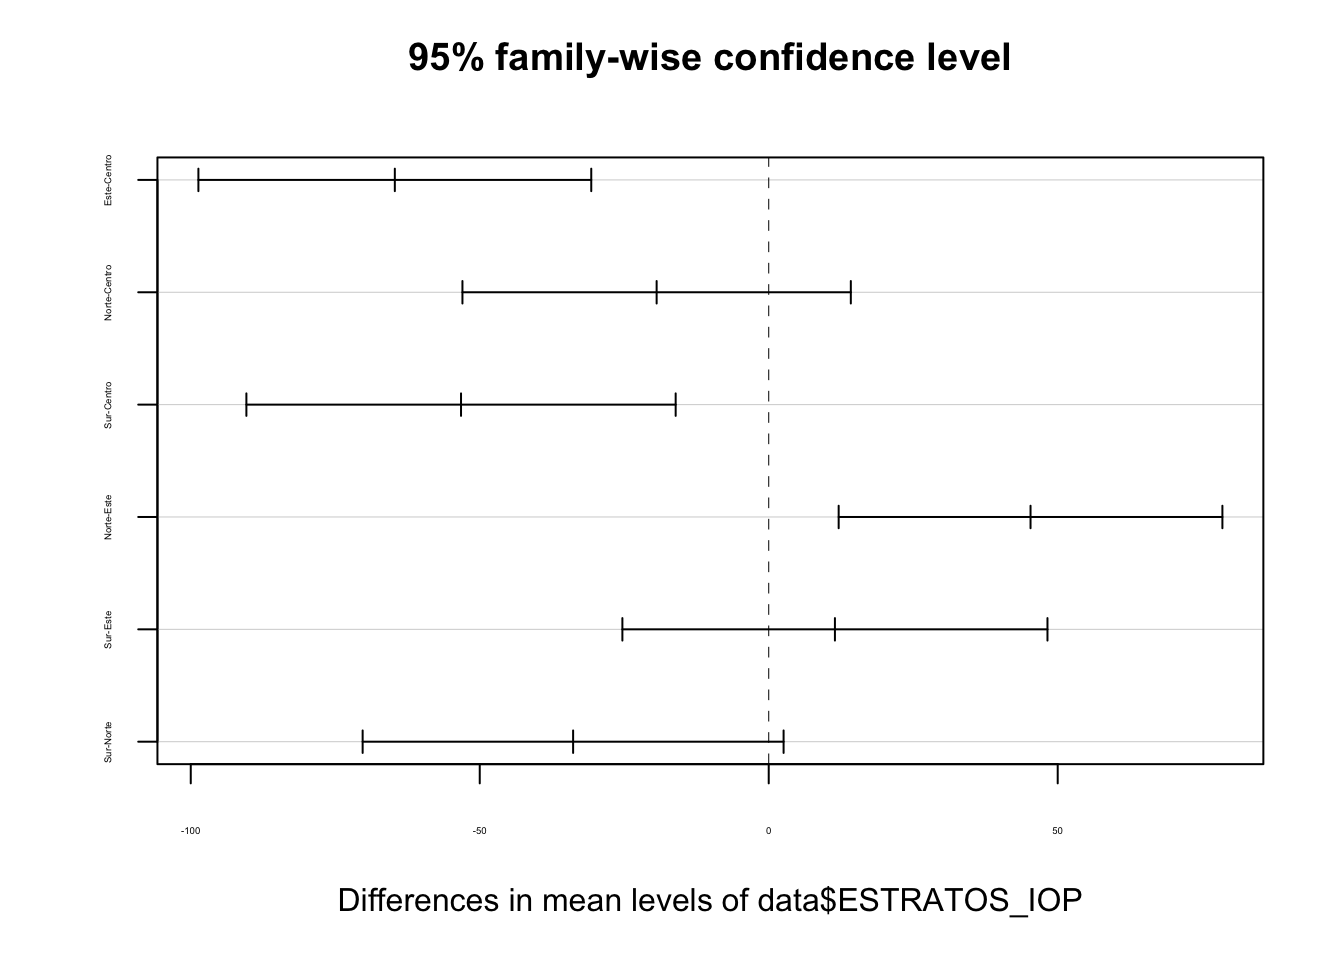
\includegraphics{pd3_files/figure-latex/unnamed-chunk-8-1.pdf}

\begin{itemize}
\tightlist
\item
  \textbf{E-Government Index}: Variable numérica
\end{itemize}

Revisamos \emph{solo} la media del E\_gov

\begin{Shaded}
\begin{Highlighting}[]
\NormalTok{data  }\SpecialCharTok{\%\textgreater{}\%} 
  \FunctionTok{summarise}\NormalTok{(}\AttributeTok{media=}\FunctionTok{mean}\NormalTok{(E\_gov))}
\end{Highlighting}
\end{Shaded}

\begin{verbatim}
##      media
## 1 58.79558
\end{verbatim}

Ahora realizamos análisis descriptivo y de dispersión. ¿Qué podemos
comentar de los datos obtenidos?

\begin{Shaded}
\begin{Highlighting}[]
\NormalTok{data  }\SpecialCharTok{\%\textgreater{}\%} 
  \FunctionTok{summarise}\NormalTok{(Mínimo}\OtherTok{=}\FunctionTok{min}\NormalTok{(E\_gov), }
            \AttributeTok{Mediana=} \FunctionTok{median}\NormalTok{(E\_gov), }
\NormalTok{            Desviación}\OtherTok{=}\FunctionTok{sd}\NormalTok{(E\_gov),}
            \AttributeTok{Media=} \FunctionTok{mean}\NormalTok{(E\_gov),}
\NormalTok{            Máximo}\OtherTok{=} \FunctionTok{max}\NormalTok{(E\_gov))}
\end{Highlighting}
\end{Shaded}

\begin{verbatim}
##   Mínimo Mediana Desviación    Media Máximo
## 1      0      59   23.98373 58.79558    100
\end{verbatim}

\begin{itemize}
\item
  ¿Cuál es el puntaje más bajo y el máximo?
\item
  ¿Cuál es el rango? (\emph{max-min})
\item
  \textbf{Desviación estándar (\emph{sd})}: \emph{La desviación estándar
  es una medida que nos ayuda a entender cuánto se separan los números
  en un conjunto de datos del valor promedio o medio. Podemos traducir
  ello como una forma de medir cuánto ``se dispersan'' los números
  alrededor de un número central.}
\item
  ¿Hay mucha variabilidad en los datos? \emph{sd}
\end{itemize}

\hypertarget{visualizaciuxf3n}{%
\subsection{\texorpdfstring{\textbf{Visualización}}{Visualización}}\label{visualizaciuxf3n}}

Histograma de E-Gov

\begin{Shaded}
\begin{Highlighting}[]
\NormalTok{data }\SpecialCharTok{\%\textgreater{}\%}
  \FunctionTok{ggplot}\NormalTok{(}\FunctionTok{aes}\NormalTok{(}\AttributeTok{x=}\NormalTok{E\_gov))}\SpecialCharTok{+}
  \FunctionTok{geom\_histogram}\NormalTok{(}\AttributeTok{fill =} \StringTok{"blue"}\NormalTok{,}
    \AttributeTok{color =} \StringTok{"black"}\NormalTok{,}
    \AttributeTok{bins =} \DecValTok{30}\NormalTok{,}
    \AttributeTok{alpha =} \FloatTok{0.7}\NormalTok{)}\SpecialCharTok{+}
  \FunctionTok{xlab}\NormalTok{(}\StringTok{"E{-}Government Index"}\NormalTok{) }\SpecialCharTok{+}
  \FunctionTok{ylab}\NormalTok{(}\StringTok{"Frecuencia"}\NormalTok{)}\SpecialCharTok{+}
   \FunctionTok{theme\_minimal}\NormalTok{()}
\end{Highlighting}
\end{Shaded}

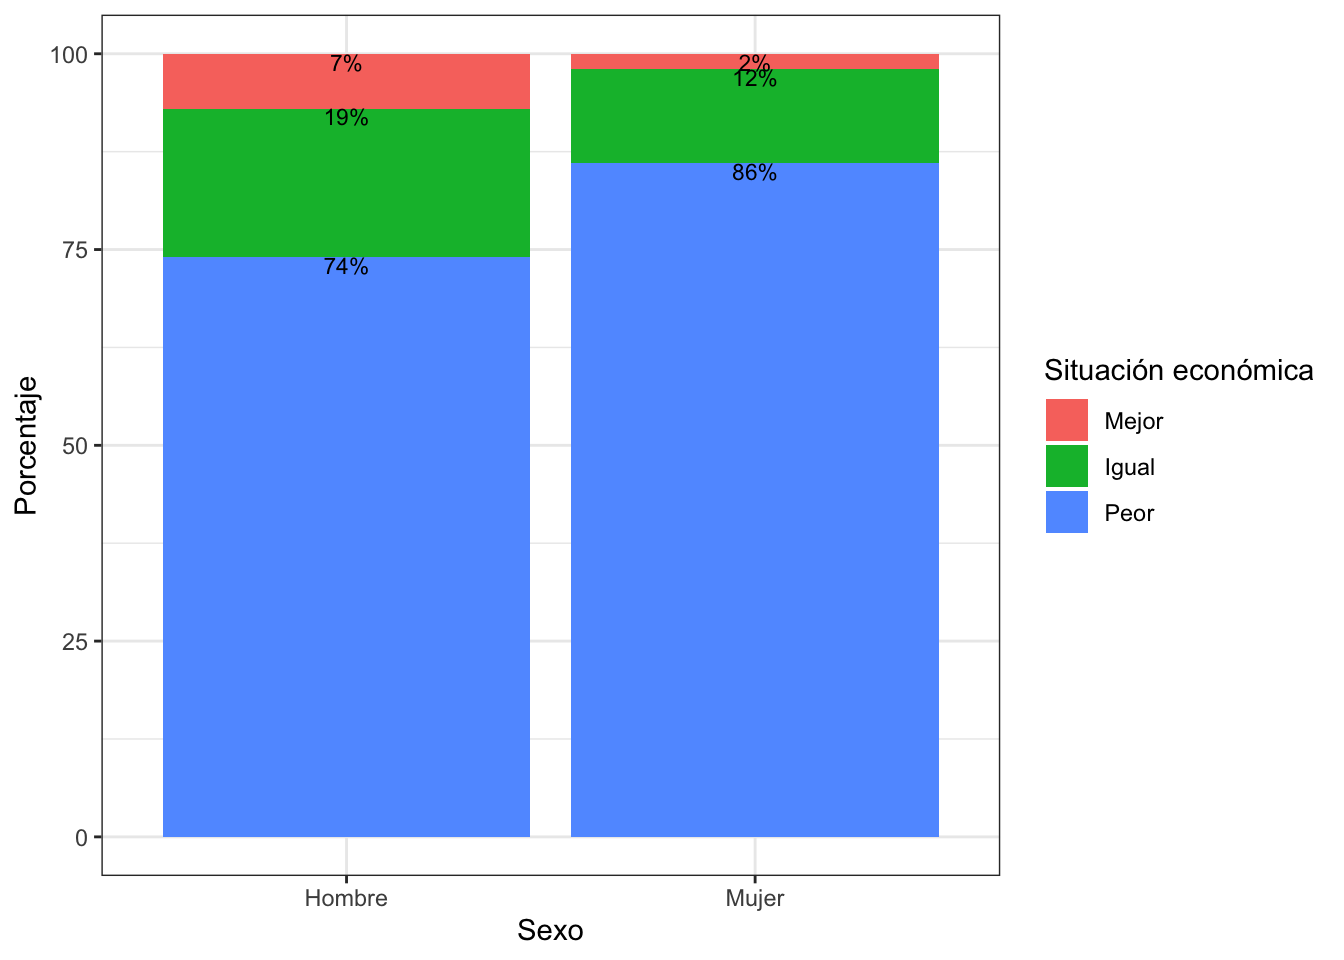
\includegraphics{pd3_files/figure-latex/unnamed-chunk-11-1.pdf}

Histograma de E-Gov + mediana (rojo) + media (verde)

\begin{Shaded}
\begin{Highlighting}[]
\NormalTok{data }\SpecialCharTok{\%\textgreater{}\%}
\FunctionTok{ggplot}\NormalTok{(}\FunctionTok{aes}\NormalTok{(}\AttributeTok{x=}\NormalTok{E\_gov))}\SpecialCharTok{+}
  \FunctionTok{geom\_histogram}\NormalTok{(}\AttributeTok{fill =} \StringTok{"blue"}\NormalTok{,}
    \AttributeTok{color =} \StringTok{"black"}\NormalTok{,}
    \AttributeTok{bins =} \DecValTok{50}\NormalTok{,}
    \AttributeTok{alpha =} \FloatTok{0.7}\NormalTok{)}\SpecialCharTok{+}
  \FunctionTok{geom\_vline}\NormalTok{(}\AttributeTok{xintercept =} \FunctionTok{median}\NormalTok{(data}\SpecialCharTok{$}\NormalTok{E\_gov), }\AttributeTok{color =} \StringTok{"red"}\NormalTok{)}\SpecialCharTok{+}
  \FunctionTok{geom\_vline}\NormalTok{(}\AttributeTok{xintercept =} \FunctionTok{mean}\NormalTok{(data}\SpecialCharTok{$}\NormalTok{E\_gov), }\AttributeTok{color =} \StringTok{"green"}\NormalTok{)}\SpecialCharTok{+}
  \FunctionTok{xlab}\NormalTok{(}\StringTok{"E{-}Government Index"}\NormalTok{) }\SpecialCharTok{+}
  \FunctionTok{ylab}\NormalTok{(}\StringTok{"Frecuencia"}\NormalTok{)}\SpecialCharTok{+}
  \FunctionTok{theme\_light}\NormalTok{()}
\end{Highlighting}
\end{Shaded}

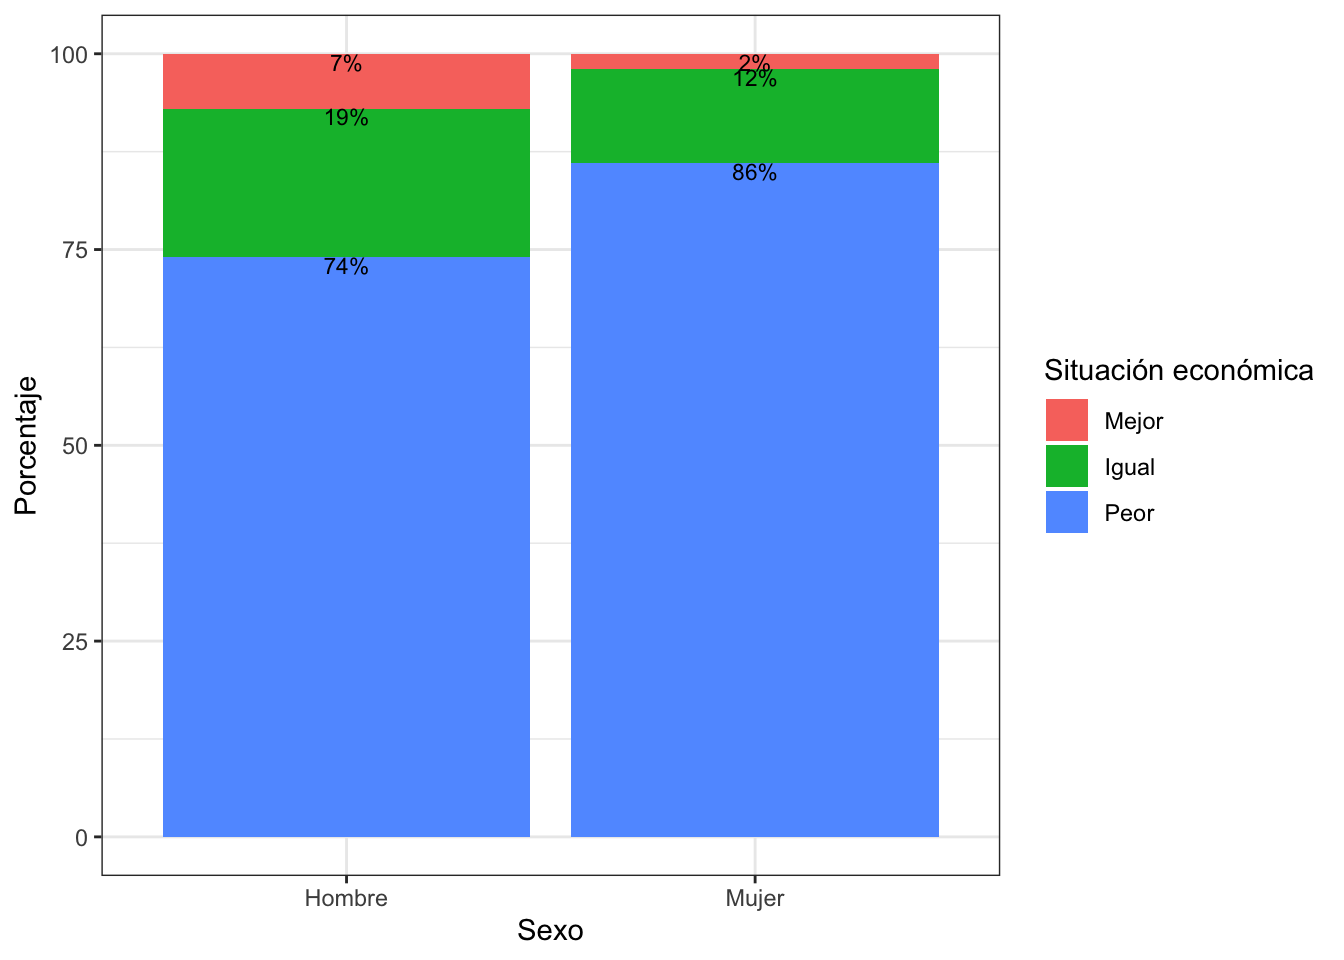
\includegraphics{pd3_files/figure-latex/unnamed-chunk-12-1.pdf}

\begin{Shaded}
\begin{Highlighting}[]
\FunctionTok{summary}\NormalTok{(data}\SpecialCharTok{$}\NormalTok{E\_gov)}
\end{Highlighting}
\end{Shaded}

\begin{verbatim}
##    Min. 1st Qu.  Median    Mean 3rd Qu.    Max. 
##     0.0    40.0    59.0    58.8    79.0   100.0
\end{verbatim}

\hypertarget{cuartiles-y-diagrama-de-cajas}{%
\subsubsection{Cuartiles y diagrama de
cajas}\label{cuartiles-y-diagrama-de-cajas}}

\begin{Shaded}
\begin{Highlighting}[]
\NormalTok{data }\SpecialCharTok{\%\textgreater{}\%} 
  \FunctionTok{filter}\NormalTok{(Region}\SpecialCharTok{==}\StringTok{"Africa"}\NormalTok{)}\SpecialCharTok{\%\textgreater{}\%} 
  \FunctionTok{summarise}\NormalTok{(}\AttributeTok{CuartilesEgov =} \FunctionTok{quantile}\NormalTok{(E\_gov))}
\end{Highlighting}
\end{Shaded}

\begin{verbatim}
##   CuartilesEgov
## 1          0.00
## 2         23.75
## 3         35.00
## 4         52.00
## 5         73.00
\end{verbatim}

\begin{Shaded}
\begin{Highlighting}[]
\NormalTok{data }\SpecialCharTok{\%\textgreater{}\%} 
  \FunctionTok{summarise}\NormalTok{(}\AttributeTok{CuartilesEgov =} \FunctionTok{quantile}\NormalTok{(E\_gov))}
\end{Highlighting}
\end{Shaded}

\begin{verbatim}
##   CuartilesEgov
## 1             0
## 2            40
## 3            59
## 4            79
## 5           100
\end{verbatim}

¿Cómo ubicamos los cuartiles en el diagrama de cajas?

\begin{Shaded}
\begin{Highlighting}[]
\NormalTok{data }\SpecialCharTok{\%\textgreater{}\%} 
  \FunctionTok{ggplot}\NormalTok{(}\FunctionTok{aes}\NormalTok{(}\AttributeTok{y=}\NormalTok{E\_gov))}\SpecialCharTok{+}
  \FunctionTok{geom\_boxplot}\NormalTok{()}\SpecialCharTok{+}
  \FunctionTok{ylab}\NormalTok{(}\StringTok{"E{-}Government Index"}\NormalTok{)}
\end{Highlighting}
\end{Shaded}

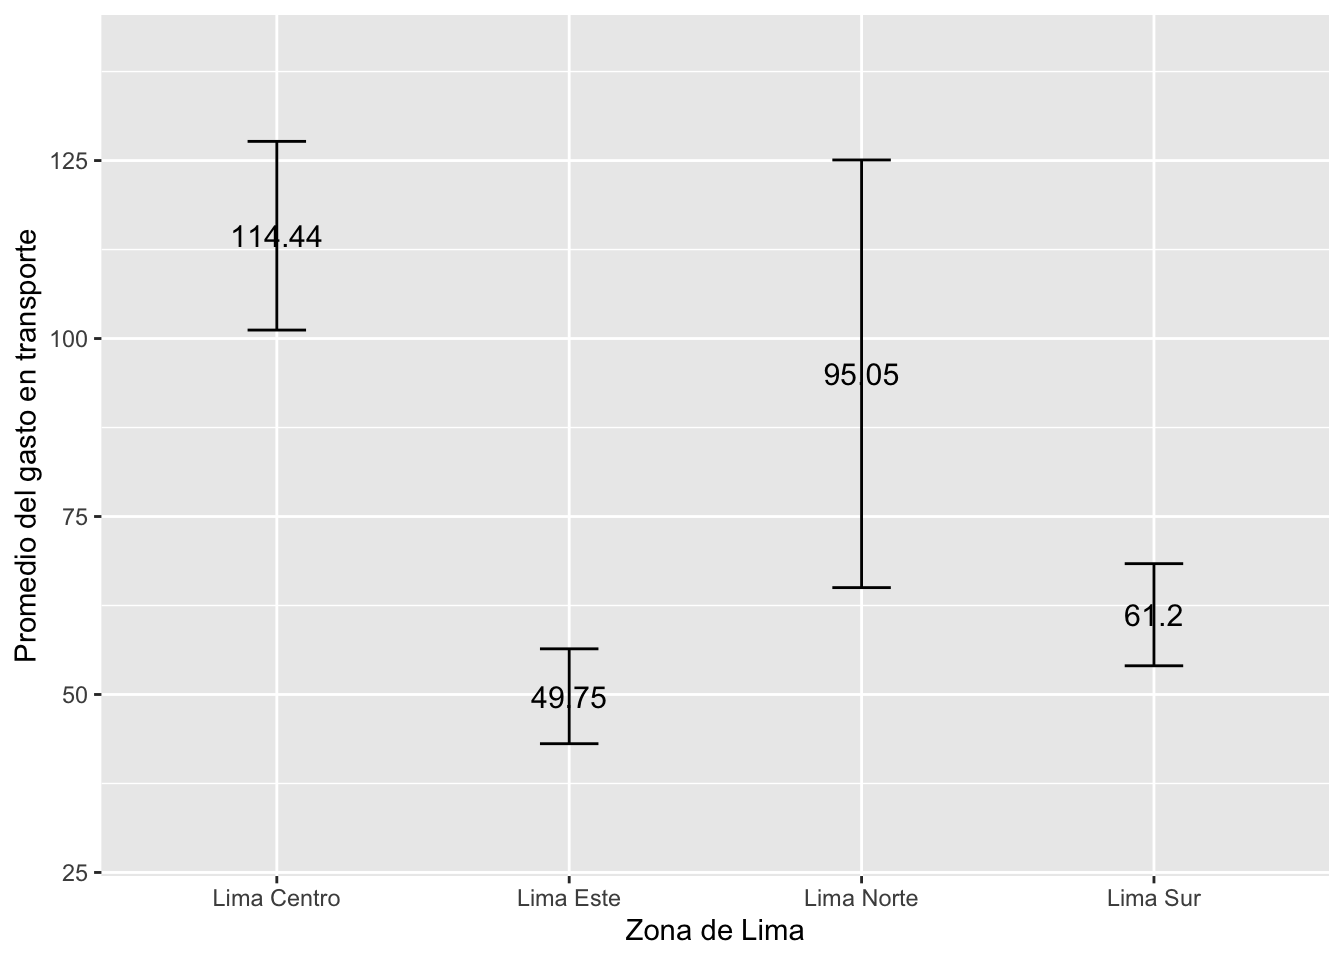
\includegraphics{pd3_files/figure-latex/unnamed-chunk-16-1.pdf}

\hypertarget{seguxfan-regiuxf3n-cuuxe1l-es-el-estado-de-la-gobernanza-digital-de-los-pauxedses}{%
\subsection{\texorpdfstring{\textbf{Según región, ¿cuál es el estado de
la gobernanza digital de los
países?}}{Según región, ¿cuál es el estado de la gobernanza digital de los países?}}\label{seguxfan-regiuxf3n-cuuxe1l-es-el-estado-de-la-gobernanza-digital-de-los-pauxedses}}

¿Cuál es la importancia de analizar por regiones?

\begin{Shaded}
\begin{Highlighting}[]
\NormalTok{data }\SpecialCharTok{\%\textgreater{}\%}
 \FunctionTok{group\_by}\NormalTok{(Region) }\SpecialCharTok{\%\textgreater{}\%}
  \FunctionTok{summarize}\NormalTok{(}\AttributeTok{Media=}\FunctionTok{mean}\NormalTok{(E\_gov)) }
\end{Highlighting}
\end{Shaded}

\begin{verbatim}
## # A tibble: 5 x 2
##   Region   Media
##   <fct>    <dbl>
## 1 Africa    36.3
## 2 Americas  62.6
## 3 Asia      63.2
## 4 Europe    84.2
## 5 Oceania   47.7
\end{verbatim}

\begin{Shaded}
\begin{Highlighting}[]
\NormalTok{data }\SpecialCharTok{\%\textgreater{}\%}
  \FunctionTok{ggplot}\NormalTok{(}\FunctionTok{aes}\NormalTok{(}\AttributeTok{x=}\NormalTok{E\_gov))}\SpecialCharTok{+}
  \FunctionTok{geom\_histogram}\NormalTok{()}\SpecialCharTok{+}
  \FunctionTok{facet\_wrap}\NormalTok{(}\SpecialCharTok{\textasciitilde{}}\NormalTok{Region)}\SpecialCharTok{+}
  \FunctionTok{xlab}\NormalTok{(}\StringTok{"E{-}Gov Index"}\NormalTok{)}\SpecialCharTok{+}
  \FunctionTok{ylab}\NormalTok{(}\StringTok{"Frecuencia"}\NormalTok{)}
\end{Highlighting}
\end{Shaded}

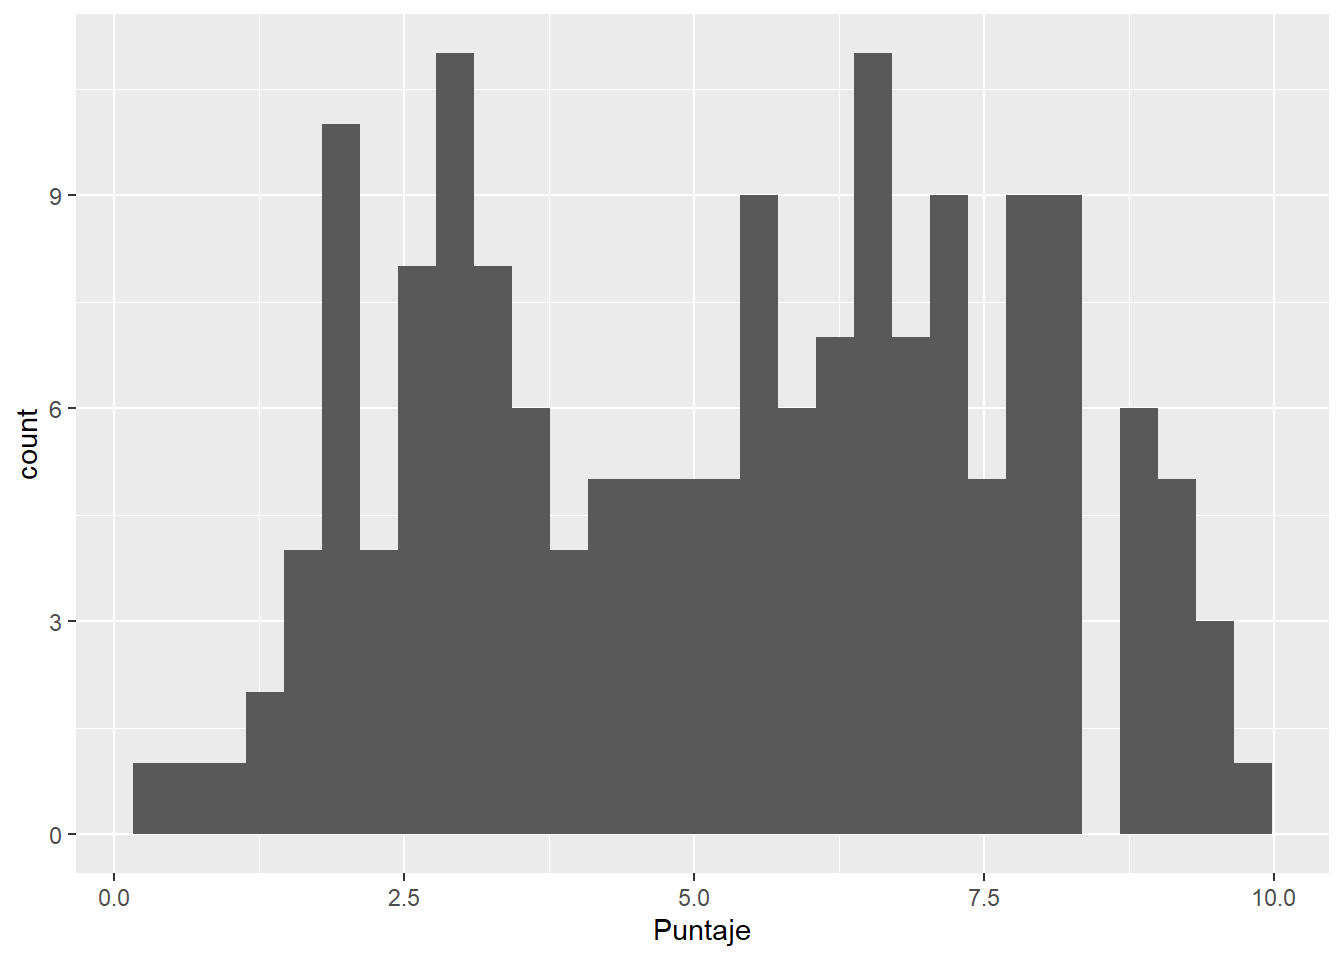
\includegraphics{pd3_files/figure-latex/unnamed-chunk-18-1.pdf}

Analicemos los resultados 😼

\textbf{Descriptivos por región}

\begin{Shaded}
\begin{Highlighting}[]
\NormalTok{ data }\SpecialCharTok{\%\textgreater{}\%}
  \FunctionTok{group\_by}\NormalTok{(Region)}\SpecialCharTok{\%\textgreater{}\%}
  \FunctionTok{summarise}\NormalTok{(Mínimo}\OtherTok{=}\FunctionTok{min}\NormalTok{(E\_gov), }
            \AttributeTok{Mediana=} \FunctionTok{median}\NormalTok{(E\_gov), }
\NormalTok{            Desviación}\OtherTok{=}\FunctionTok{sd}\NormalTok{(E\_gov),}
            \AttributeTok{Media=} \FunctionTok{mean}\NormalTok{(E\_gov),}
\NormalTok{            Máximo}\OtherTok{=} \FunctionTok{max}\NormalTok{(E\_gov))}
\end{Highlighting}
\end{Shaded}

\begin{verbatim}
## # A tibble: 5 x 6
##   Region   Mínimo Mediana Desviación Media Máximo
##   <fct>     <dbl>   <dbl>      <dbl> <dbl>  <dbl>
## 1 Africa        0    35        17.3   36.3     73
## 2 Americas     18    62.5      15.5   62.6     86
## 3 Asia         21    67        19.3   63.2     93
## 4 Europe       61    86         9.35  84.2    100
## 5 Oceania      27    40.5      22.6   47.7     97
\end{verbatim}

Comparo los resultados y los ubico en mi diagrama de cajas

\begin{Shaded}
\begin{Highlighting}[]
\NormalTok{ data }\SpecialCharTok{\%\textgreater{}\%}
\FunctionTok{ggplot}\NormalTok{(}\FunctionTok{aes}\NormalTok{(}\AttributeTok{x=}\NormalTok{Region, }\AttributeTok{y=}\NormalTok{E\_gov, }\AttributeTok{color=}\NormalTok{Region)) }\SpecialCharTok{+} 
  \FunctionTok{geom\_boxplot}\NormalTok{() }\SpecialCharTok{+} 
  \FunctionTok{geom\_jitter}\NormalTok{(}\AttributeTok{shape=}\DecValTok{16}\NormalTok{, }\AttributeTok{position=}\FunctionTok{position\_jitter}\NormalTok{(}\FloatTok{0.2}\NormalTok{)) }\SpecialCharTok{+}\CommentTok{\#para agregar los casos como puntos}
  \FunctionTok{theme\_classic}\NormalTok{()}
\end{Highlighting}
\end{Shaded}

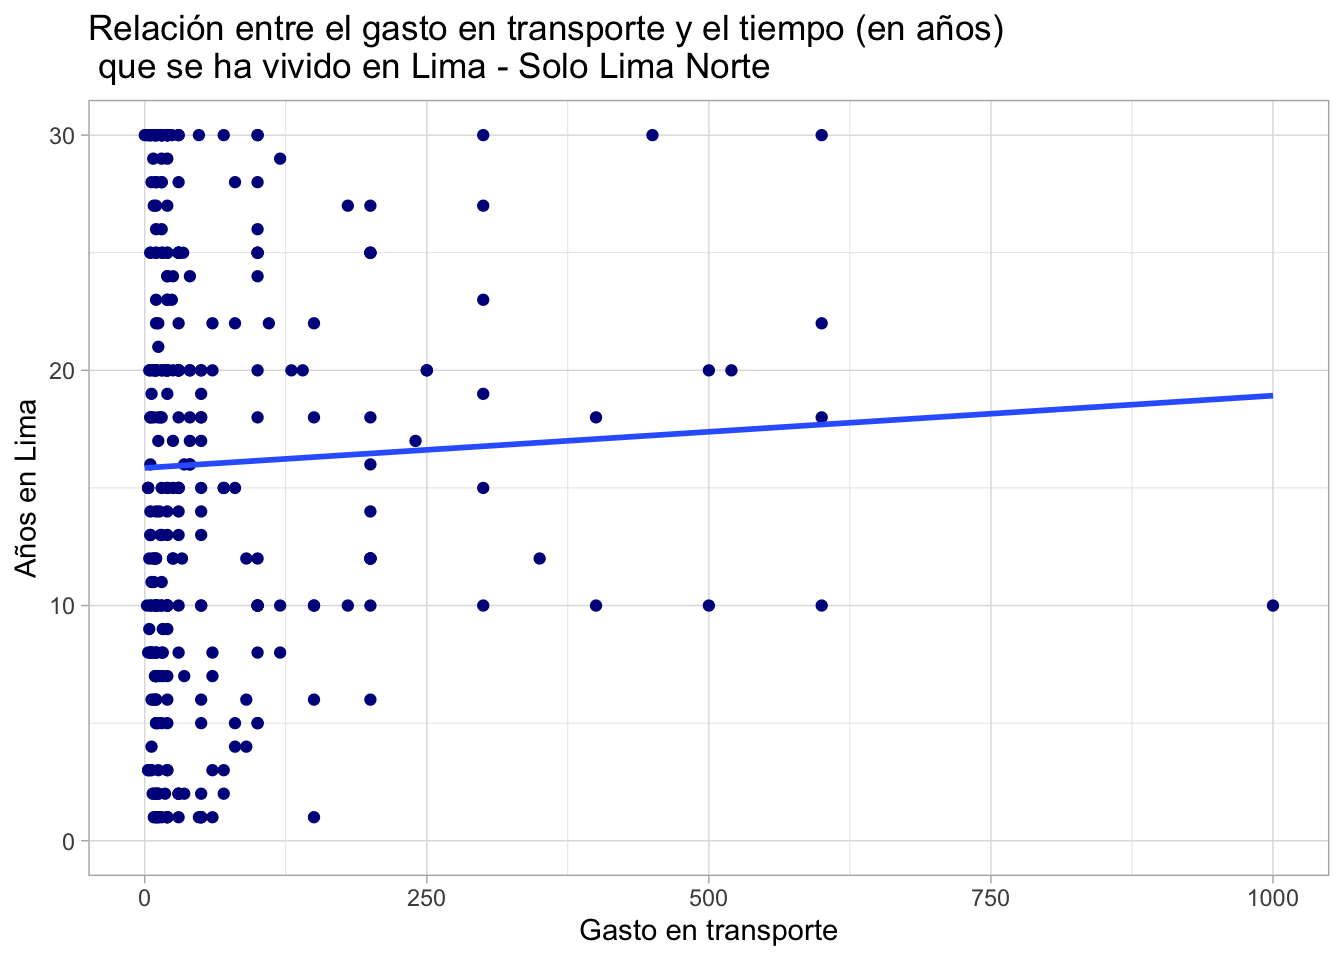
\includegraphics{pd3_files/figure-latex/unnamed-chunk-20-1.pdf}

Si deseo un subset solamente de los países que están por encima de la
media ¿cuántos países son?

\begin{Shaded}
\begin{Highlighting}[]
\NormalTok{MayorMedia}\OtherTok{=}\NormalTok{data }\SpecialCharTok{\%\textgreater{}\%}
  \FunctionTok{filter}\NormalTok{(E\_gov }\SpecialCharTok{\textgreater{}} \FunctionTok{mean}\NormalTok{(E\_gov)) }
\end{Highlighting}
\end{Shaded}

Si queremos ver solo una región, en este caso África

\begin{Shaded}
\begin{Highlighting}[]
\NormalTok{data }\SpecialCharTok{\%\textgreater{}\%} 
  \FunctionTok{filter}\NormalTok{(Region }\SpecialCharTok{==}\StringTok{"Africa"}\NormalTok{) }\SpecialCharTok{\%\textgreater{}\%}
  \FunctionTok{summarise}\NormalTok{(}\FunctionTok{mean}\NormalTok{(E\_gov))}
\end{Highlighting}
\end{Shaded}

\begin{verbatim}
##   mean(E_gov)
## 1    36.28846
\end{verbatim}

O los estadísticos de los países de Asia

\begin{Shaded}
\begin{Highlighting}[]
\NormalTok{data }\SpecialCharTok{\%\textgreater{}\%}
  \FunctionTok{filter}\NormalTok{(Region }\SpecialCharTok{==} \StringTok{"Asia"}\NormalTok{) }\SpecialCharTok{\%\textgreater{}\%}
  \FunctionTok{summarise}\NormalTok{(Mínimo}\OtherTok{=}\FunctionTok{min}\NormalTok{(E\_gov), }
            \AttributeTok{Mediana=} \FunctionTok{median}\NormalTok{(E\_gov), }
\NormalTok{            Desviación}\OtherTok{=}\FunctionTok{sd}\NormalTok{(E\_gov),}
            \AttributeTok{Media=} \FunctionTok{mean}\NormalTok{(E\_gov),}
\NormalTok{            Máximo}\OtherTok{=} \FunctionTok{max}\NormalTok{(E\_gov))}
\end{Highlighting}
\end{Shaded}

\begin{verbatim}
##   Mínimo Mediana Desviación    Media Máximo
## 1     21      67   19.31929 63.16279     93
\end{verbatim}

\hypertarget{ejercicios}{%
\section{\texorpdfstring{\textbf{3. Ejercicios 👾
:}}{3. Ejercicios 👾 :}}\label{ejercicios}}

\begin{itemize}
\tightlist
\item
  Realizar los estadísticos descriptivos del Online Service Index
  (Online\_Service).
\item
  Realizar una muestra de aquellos paises que están por encima de la
  media del índice de infraestructura y telecomunicaciones
  (Tele\_infra).
\item
  Realizar diagrama de cajas del E-Participation Index (E\_part) por
  región.
\item
  Según si tiene alto nivel de infraestructura en telecomunicaciones
  (Alto\_teleinfra), calcula los cuartiles de la variable Human\_cap, y
  luego genera un gráfico que los muestre.
\end{itemize}

\end{document}
